\subsection{Simulation}

\begin{frame}
\begin{center}
	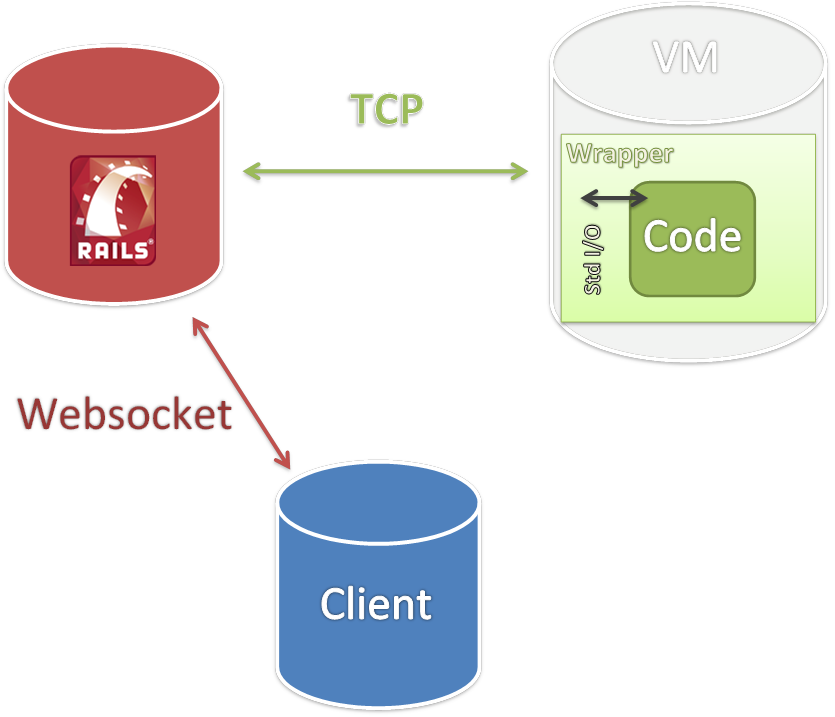
\includegraphics[scale=0.35]{overview}
\end{center}
\end{frame}

\begin{frame}
	\begin{center}
		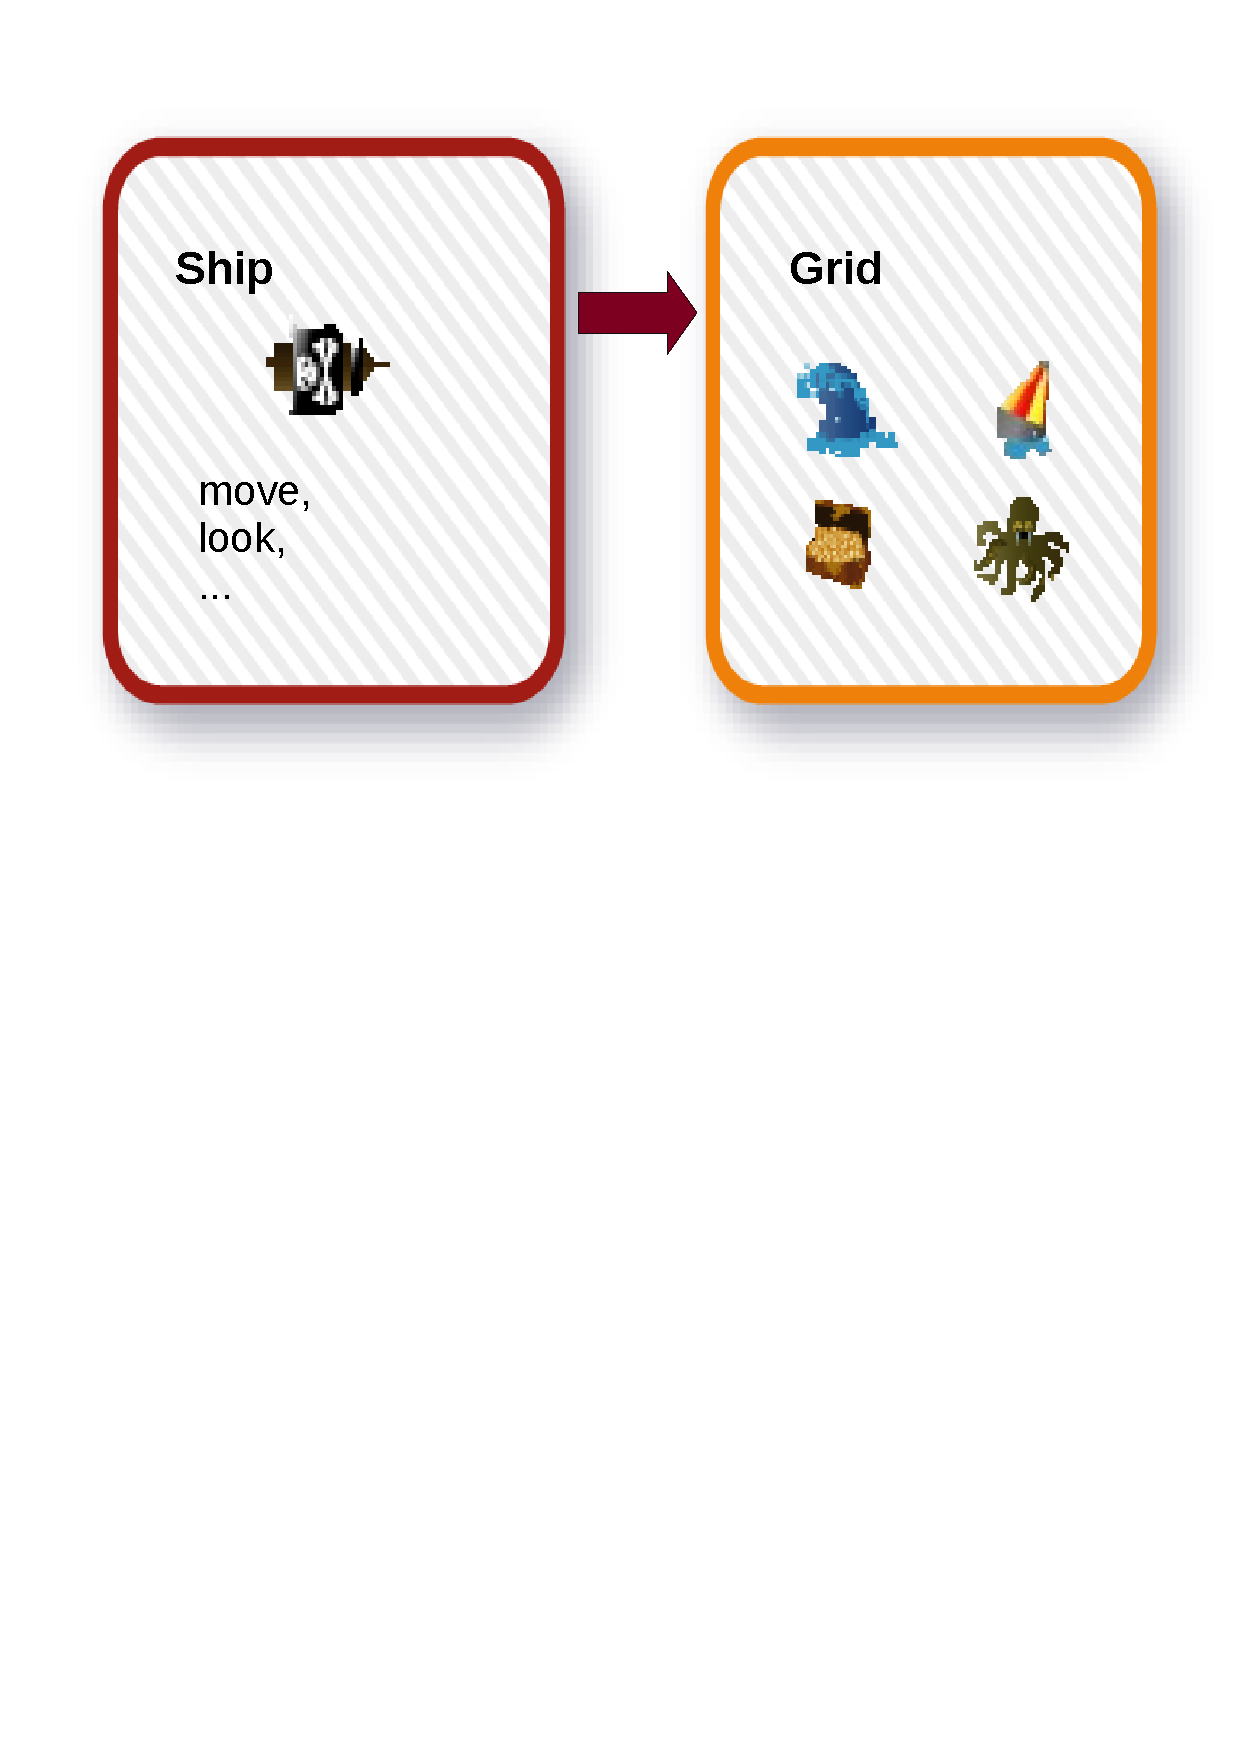
\includegraphics[scale=0.5]{simulation/Simulation6.pdf}
	\end{center}
	%Die Simulation ist der aktuelle Zustand des Systems. wir die aufteilung in Grid und Ship. Im Grid liegen nur die Objekte auf unserem Spielfeld unter ihren Koordinaten gespeichert. Die Ausführung ist stehts aus Sicht des Schiffes. Hier haben wir die ganzen Funktionen. Wir lesen die Ausgaben der VM aus und rufen die entsprechenden Funktionen auf. Dadurch ist die Simulation komplett Sprachunabhängig. Aus der Simulation können wir die VM stoppen und schicken alle wichtigen Daten per Paket an die GUI. 
\end{frame}

\begin{frame}
	\begin{center}
		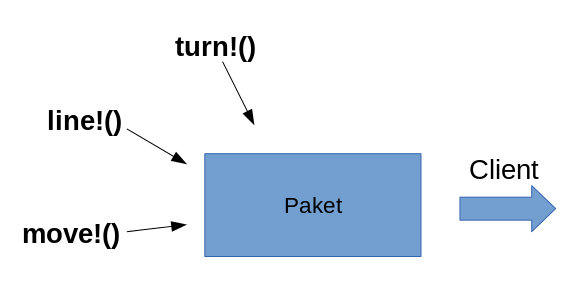
\includegraphics[scale=0.5]{simulation/Pakete.jpg}
	\end{center}
	%Für jede Zeile des ursprünglichen Codes wird ein Paket gepackt, in die jede aufgerufene Funktion Informationen für den Server packen können. Ist man am Ende einer Zeile angelangt, wird das Paket losgeschickt. 
\end{frame}


\begin{frame}
	\begin{center}
		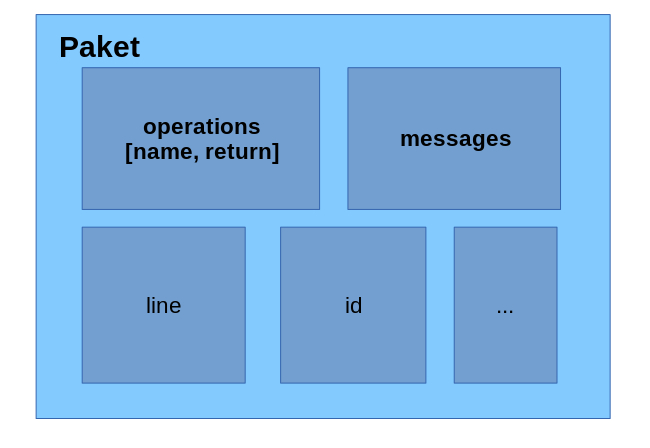
\includegraphics[scale=0.5]{simulation/Pakete2.jpg}
	\end{center}
	%Wir stellen verschiedene Paketschlüssel zur verfügung, am wichtigsten für die Simulation ist message und operations. Über Operations werden Funktionen beim Client aufgerufen und mit Message werden Nachrichten an den User übergeben. Bei look würden wir zb. ein operation-Paketelement erstellen mit name= look und return = zu highlightende Koordinate und nicht Element an dieser Koordinate -> das wird nicht benötigt.
\end{frame}